\begin{figure}[htbp]
\centering
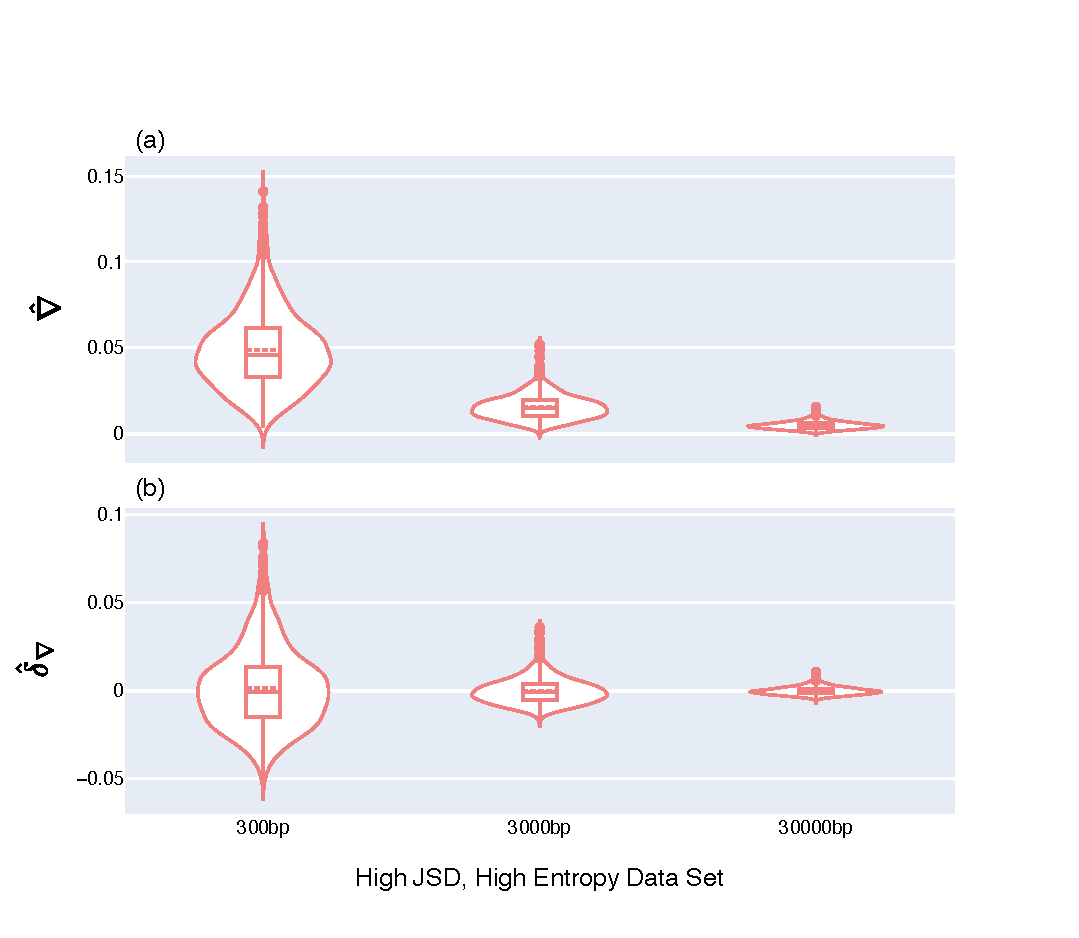
\includegraphics[width=\textwidth]{figures/plots/synthetic/d-conv-vs-conv/High JSD, High Entropy.pdf}
\caption{\textbf{The transformed statistic, $\delta_\nabla$, corrects for error introduced by the length of the alignment.} The violin plots show the distribution of $\hat \delta_\nabla$ for simulated data sets of alignment length 300, 3,000, and 30,000. \textbf{(a)} The original statistic, $\nabla$, had both a higher level of variation and a higher expected value in shorter sequences. \textbf{(b)} The transformed statistic $\delta_\nabla$ corrects for the location of the expected value only. The variation in shorter sequences remains, however, the mean for alignments of all lengths is centred on zero. Each data set contains 1,000 synthetic stationary alignments. The High JSD, High Entropy seed is shown, however, this result was the same for all seeds, included in the appendix (see Figure \ref{fig:synthetic/conv/all_seeds}). }
\label{fig:synthetic/d-conv-vs-conv/HighJSDHighEntropy}
\end{figure}